\documentclass[14pt,a4paper]{extreport}

\usepackage[utf8]{inputenc}
\usepackage[romanian]{babel}

% \renewcommand\familydefault{\sfdefault} % computer modern sans serif
\usepackage{fontspec}
\setmainfont{Times New Roman}


\linespread{1}

\usepackage{geometry}
 \geometry{
 left=20mm,
 right=10mm,
 top=20mm,
 bottom=20mm,
 % showframe
}

\usepackage{xcolor}
\definecolor{mygreen}{rgb}{0,0.6,0}
\definecolor{mygray}{rgb}{0.5,0.5,0.5}
\definecolor{mymauve}{rgb}{0.58,0,0.82}
\definecolor{darkgray}{rgb}{.4,.4,.4}
\definecolor{navy}{HTML}{000080}
\definecolor{purple}{rgb}{0.65, 0.12, 0.82}
\definecolor{codepurple}{rgb}{0.58,0,0.82}
\definecolor{backcolour}{rgb}{0.95,0.95,0.92}

\usepackage{listings}
\definecolor{codegreen}{rgb}{0,0.6,0}
\definecolor{codegray}{rgb}{0.5,0.5,0.5}
\definecolor{codepurple}{rgb}{0.58,0,0.82}
\definecolor{backcolour}{rgb}{0.95,0.95,0.95}

\lstset{
    backgroundcolor=\color{backcolour},   
    commentstyle=\color{codegreen},
    keywordstyle=\color{magenta},
    numberstyle=\color{navy},
    stringstyle=\color{codepurple},
    breakatwhitespace=false,         
    breaklines=true,                 
    captionpos=b,                    
    keepspaces=true,                 
    numbers=left,                    
    numbersep=5pt,                  
    showspaces=false,                
    showstringspaces=false,
    showtabs=false,                  
    tabsize=2,
  columns=fullflexible,
  frame=single,
  breaklines=true,
  postbreak=\mbox{\textcolor{red}{$\hookrightarrow$}\space},
}

% Please add the following required packages to your document preamble:
\usepackage{multirow}
\usepackage{array}

\usepackage{caption}
% \usepackage[singlelinecheck=false]{caption}

% \captionsetup[table]{name=Tabelul}

\usepackage{graphicx}
\graphicspath{ {./fig/} }

\usepackage{amsmath} % for the equation* environment
\usepackage{biblatex}
% \addbibresource{reference.bib}
\usepackage{blindtext}
\usepackage{hyperref}

\begin{document}

\begin{titlepage}
\begin{center}
	{\large{ Universitatea Tehnica a Moldovei \\}}
	{\large{ Facultatea Calculatoare, Informatică și Microelectronică \\}}
	{\large{ Departamentul Ingineria Software și Automatică \\}}
	\vspace{4cm}
	{\LARGE {\bf{ Raport }}}\\
	\vspace{1cm}
	{\large { Lucrarea de Laborator Nr.4 \\}}
	{\large { Metode și Modele de Calcul – 2 \\}}
	{\large { Tema: Probleme de Programare Liniara \\}}
\end{center}

\vspace{5cm}

\noindent{\large A efectuat:\hfill St. gr. TI-206} \\
\noindent{\large\null\hfill Pleșu Cătălin} \\
\noindent{\null} \\
\noindent{\large A verificat:\hfill Asist. Univ.} \\
\noindent{\large\null\hfill O. Buldumac} \\

\vspace{5cm}

\centering{\large{ Chișinău 2021 }}
\end{titlepage}


\clearpage
\subsection*{Scopul:\\}
Minimizarea și maximizarea problemelor de programare liniară.

\subsection*{Sarcina:}
\begin{enumerate}
	\item De formulat două probleme de programare liniară.
	\item PL minimizare - problema dietei.
	\item PL maximizare - producție.
	\item De modelat matematic problemele.
	\item De rezolvat problemele analitic pe foaie.
	\item De rezolvat problemele prin intermediul unei librării pentru un 
		limbaj de programare la alegere.
probleme.
\end{enumerate}

\clearpage
\subsection*{PPL de Minimizare – dietă}
\paragraph{}
Un student poate găti doar cartofi, piept de gaină, hriscă și ouă. Să se elaboreze o dietă cât mai echilibrată astfel încât studentul să stupravețuiasca pană în semestrul următor. Datele problemei sunt în tabelul de mai jos.


\paragraph{}
\begin{figure}[h]
\begin{center}
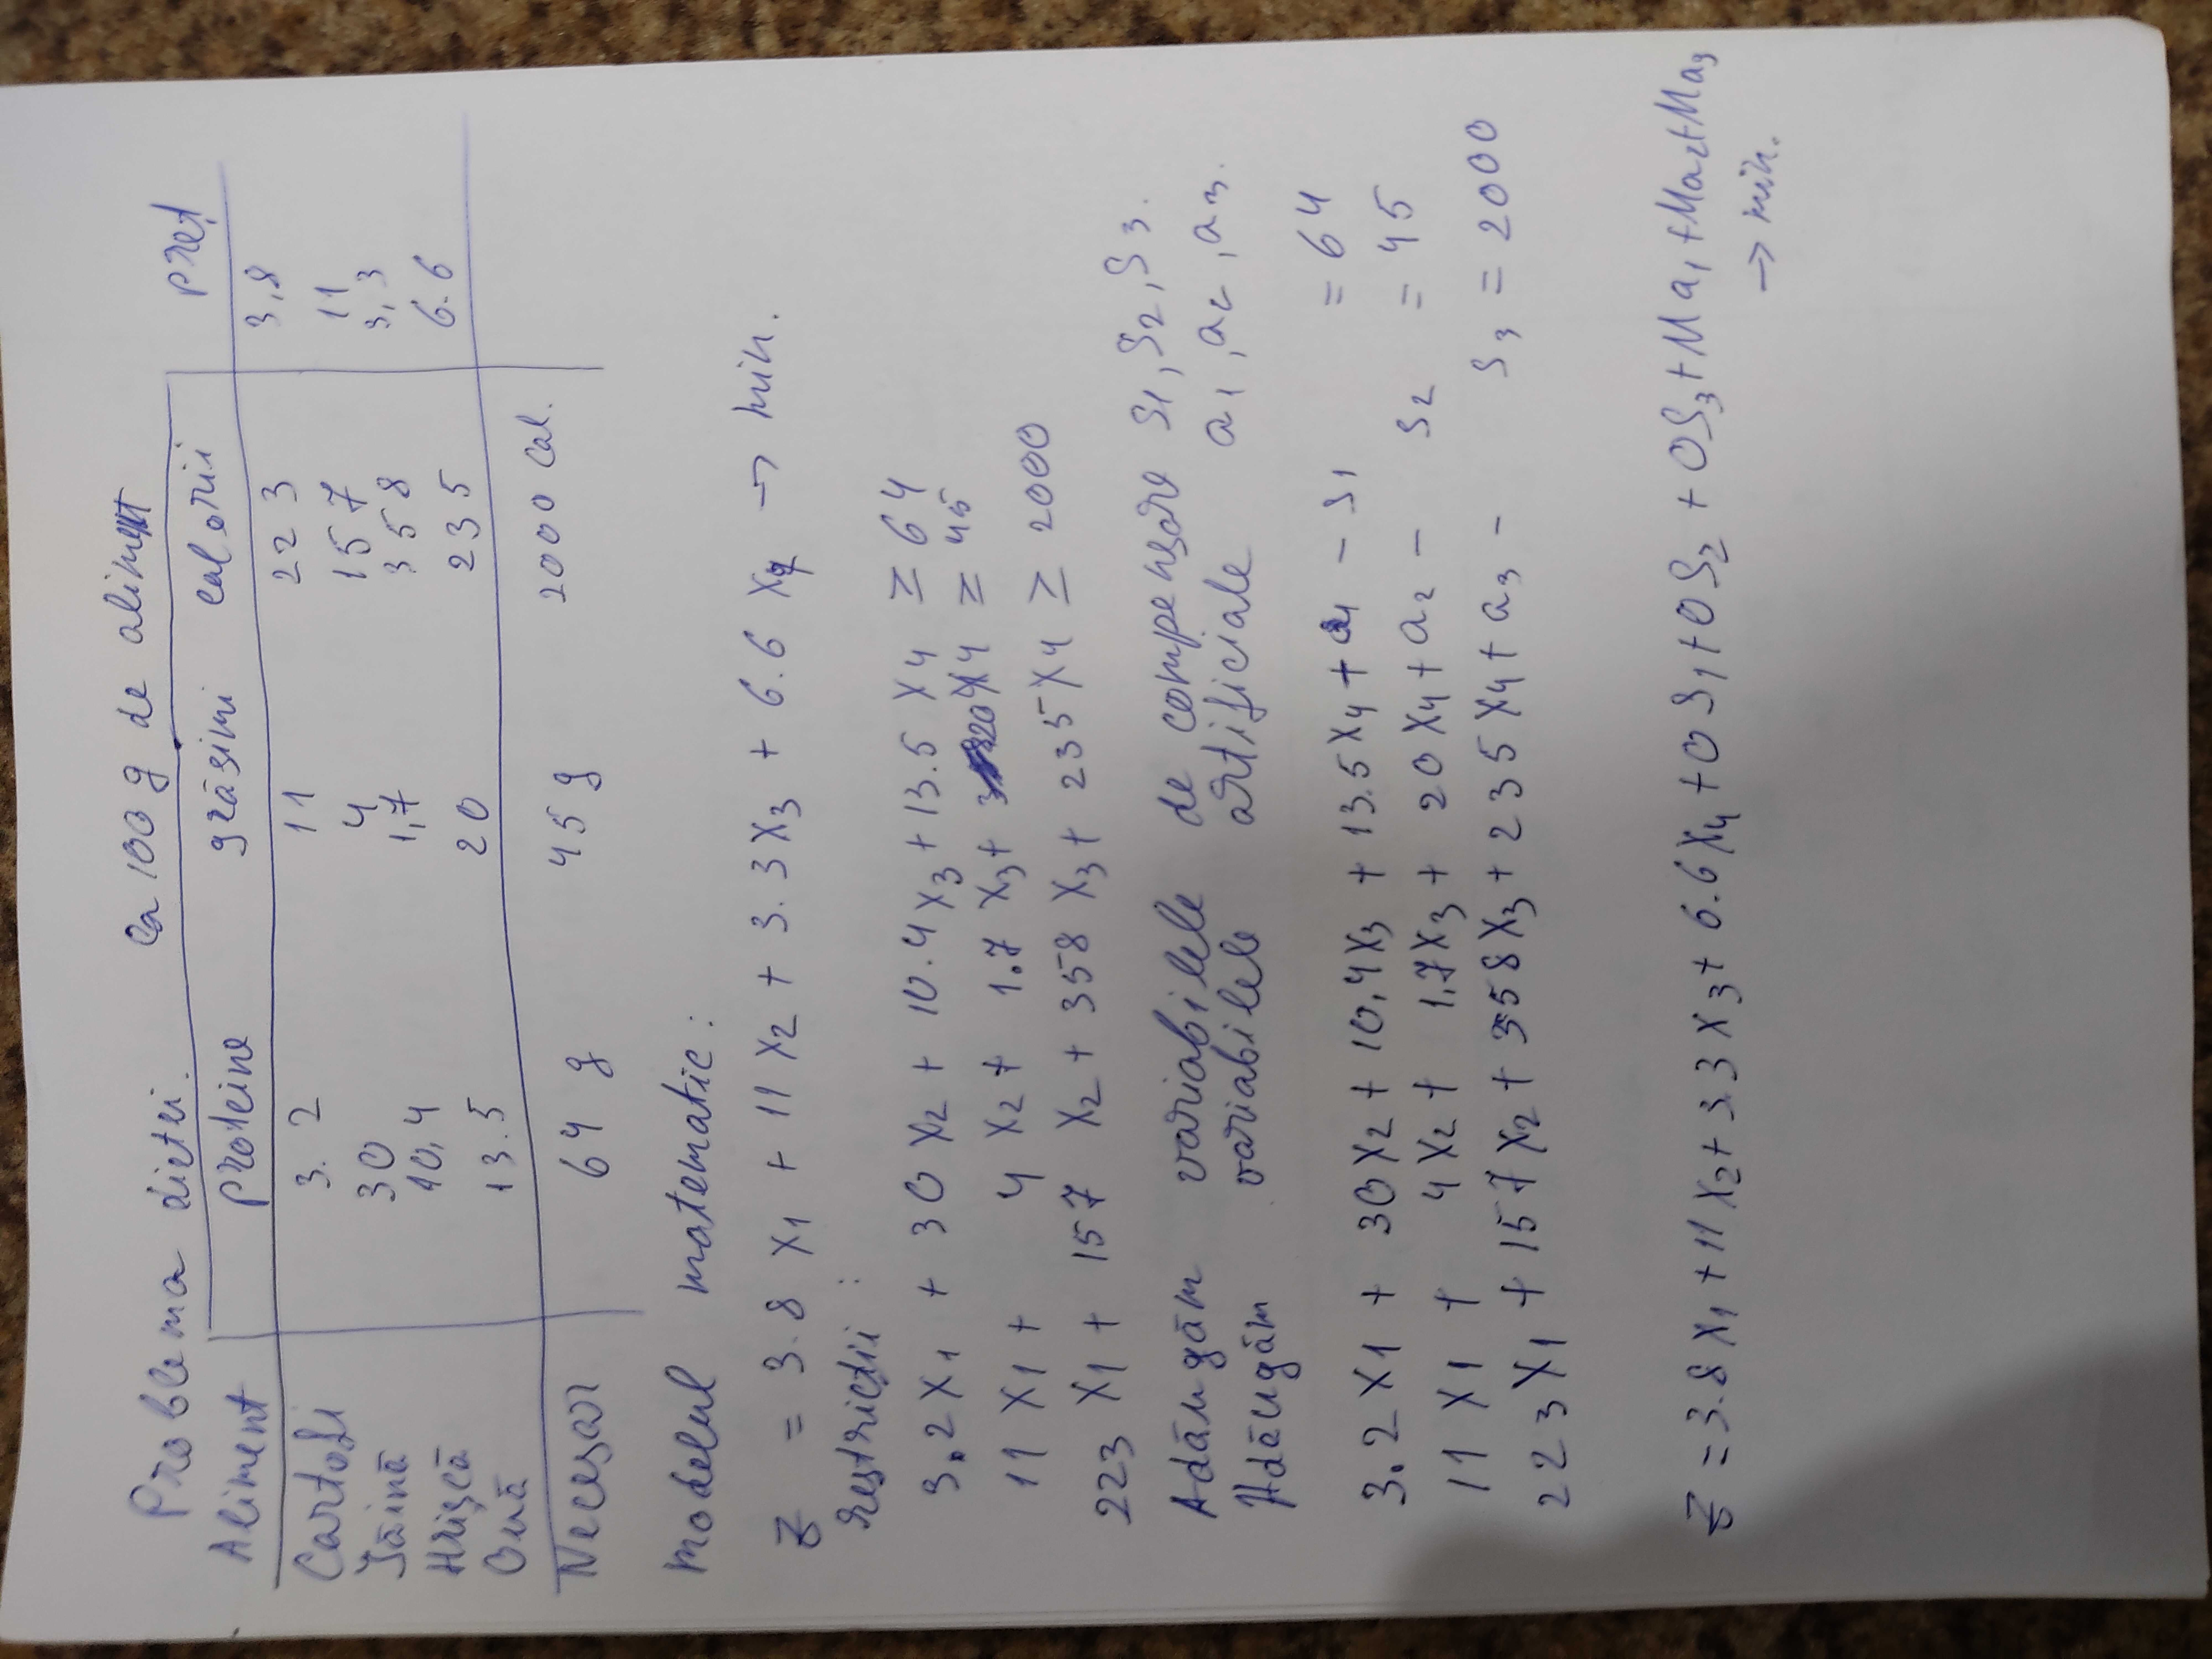
\includegraphics[width=22cm, angle =-90]{3}
\caption{Datele problemei și modelul matematic} 
\label{fig:3}
\end{center}
\end{figure}

\paragraph{}
\begin{figure}[h]
\begin{center}
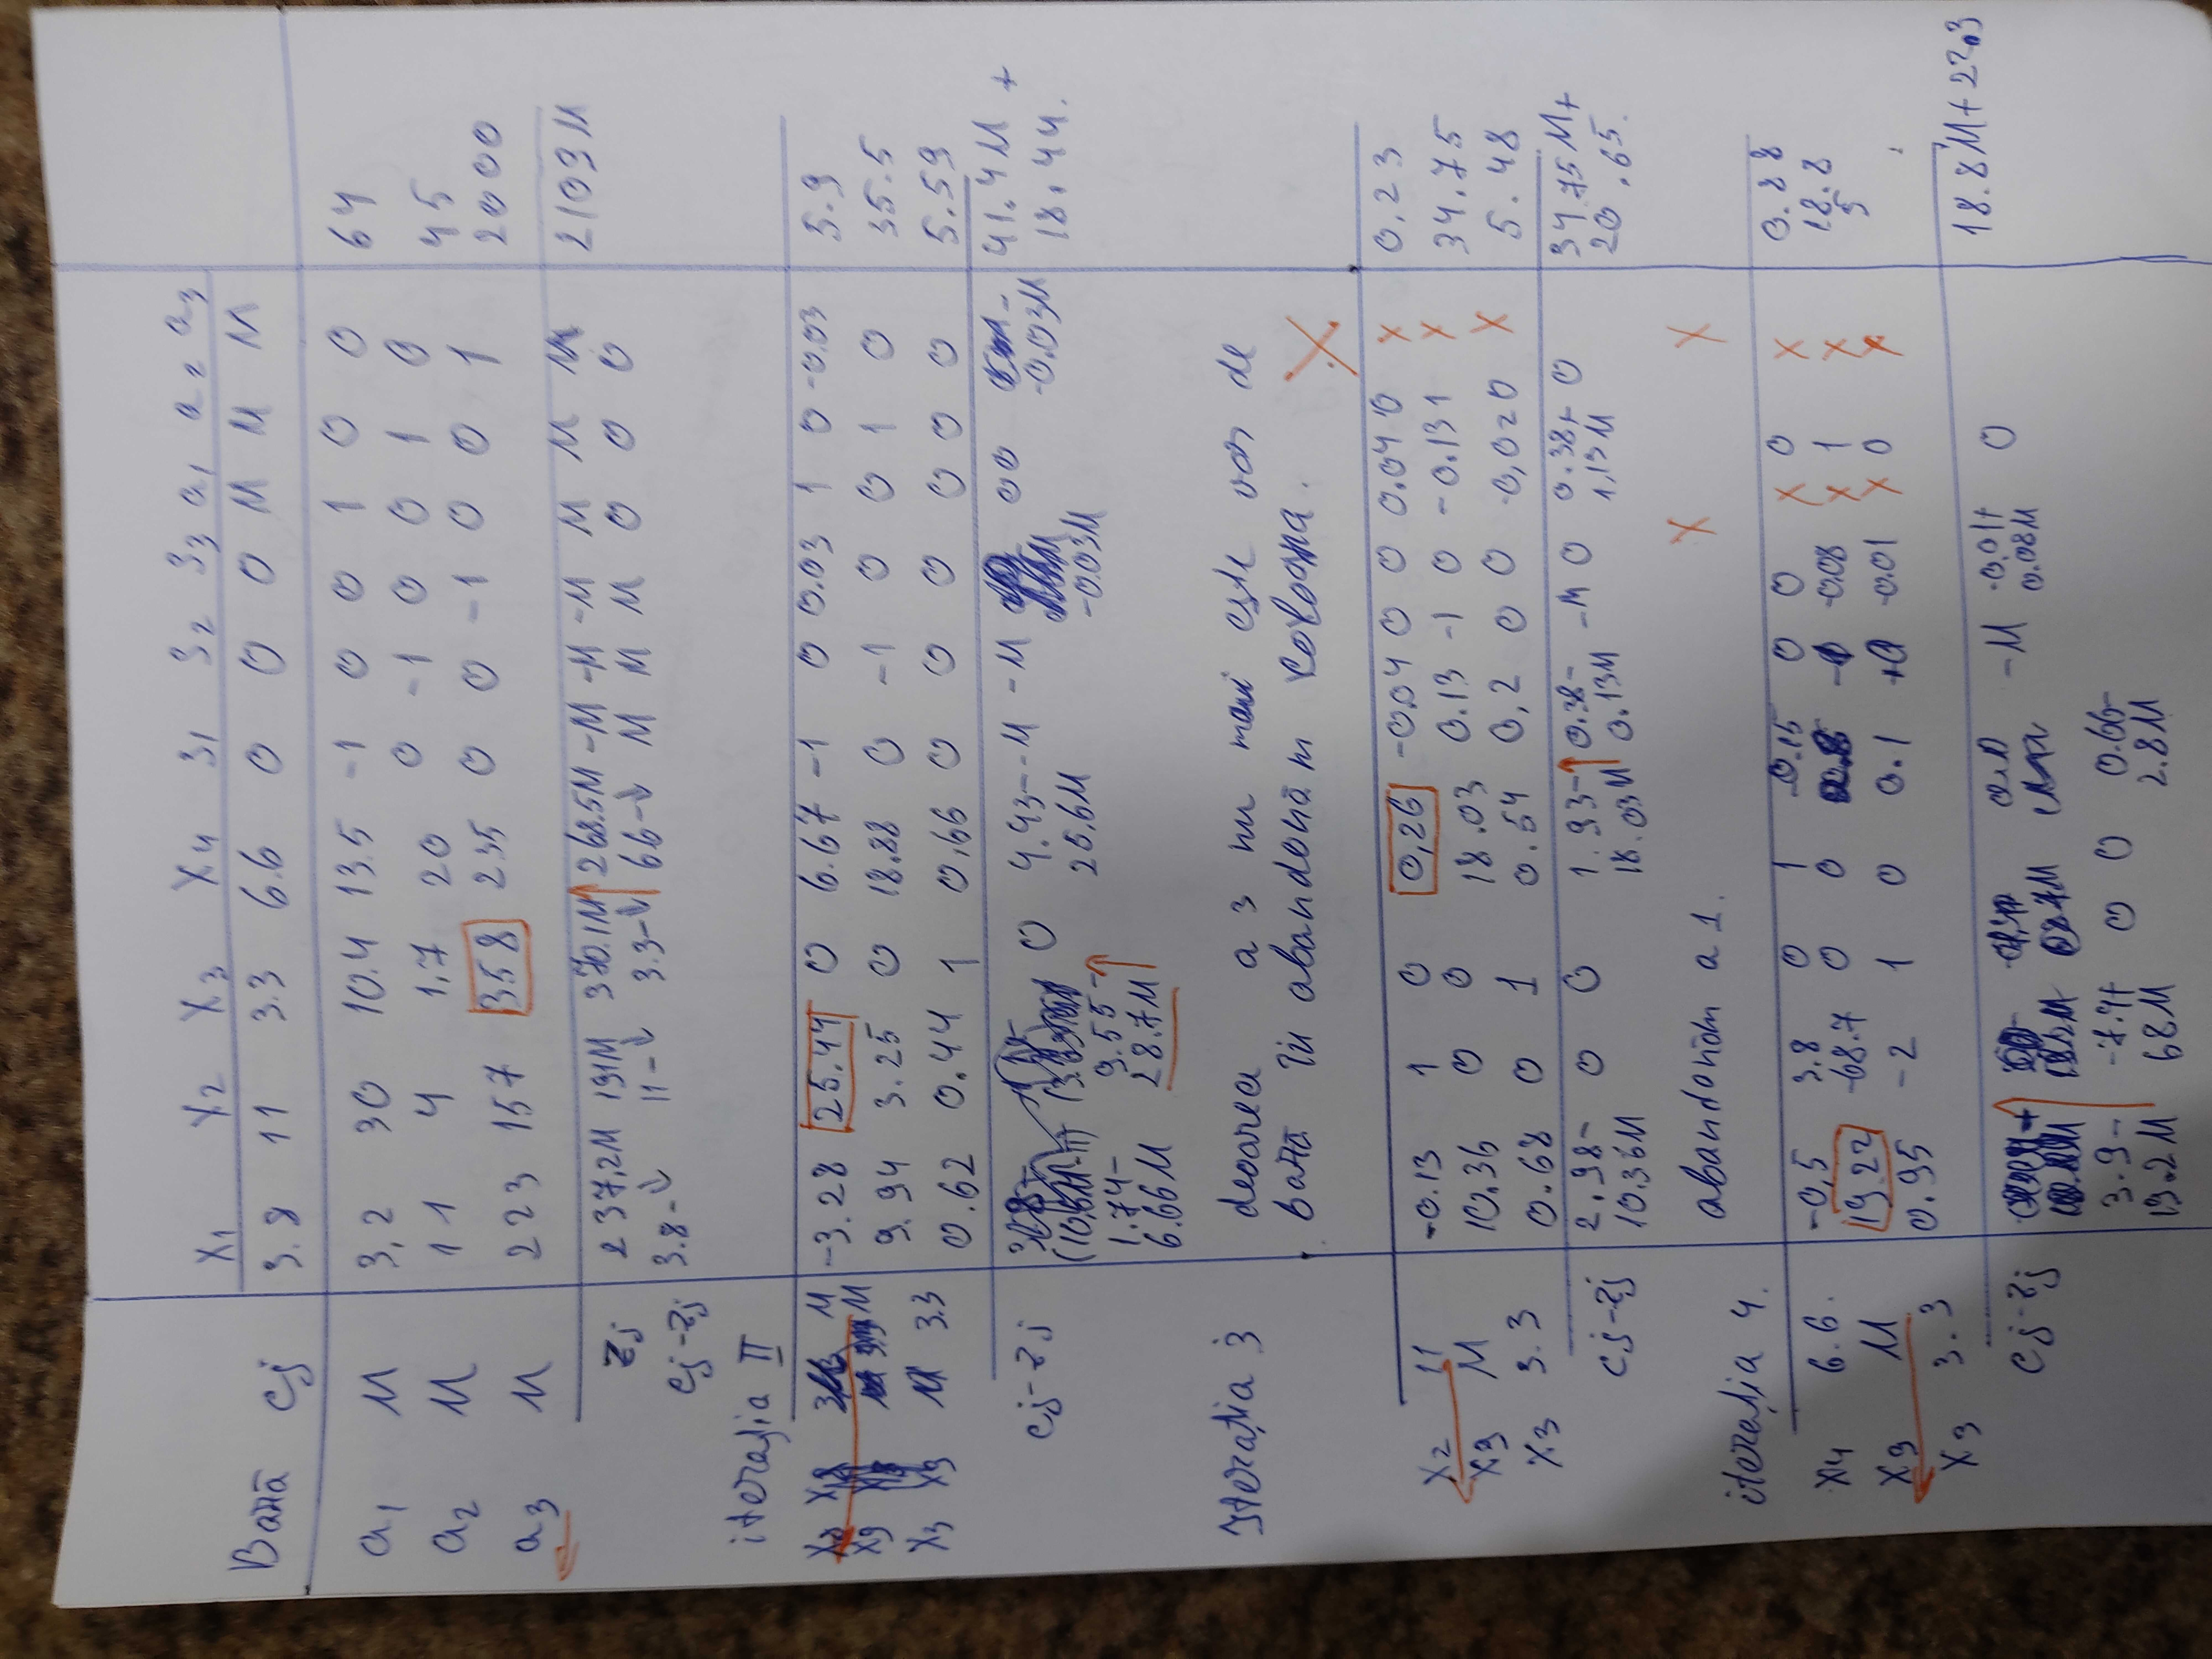
\includegraphics[width=22cm, angle =-90]{4}
\caption{Metoda simplex} 
\label{fig:4}
\end{center}
\end{figure}


\paragraph{}
\begin{figure}[h]
\begin{center}
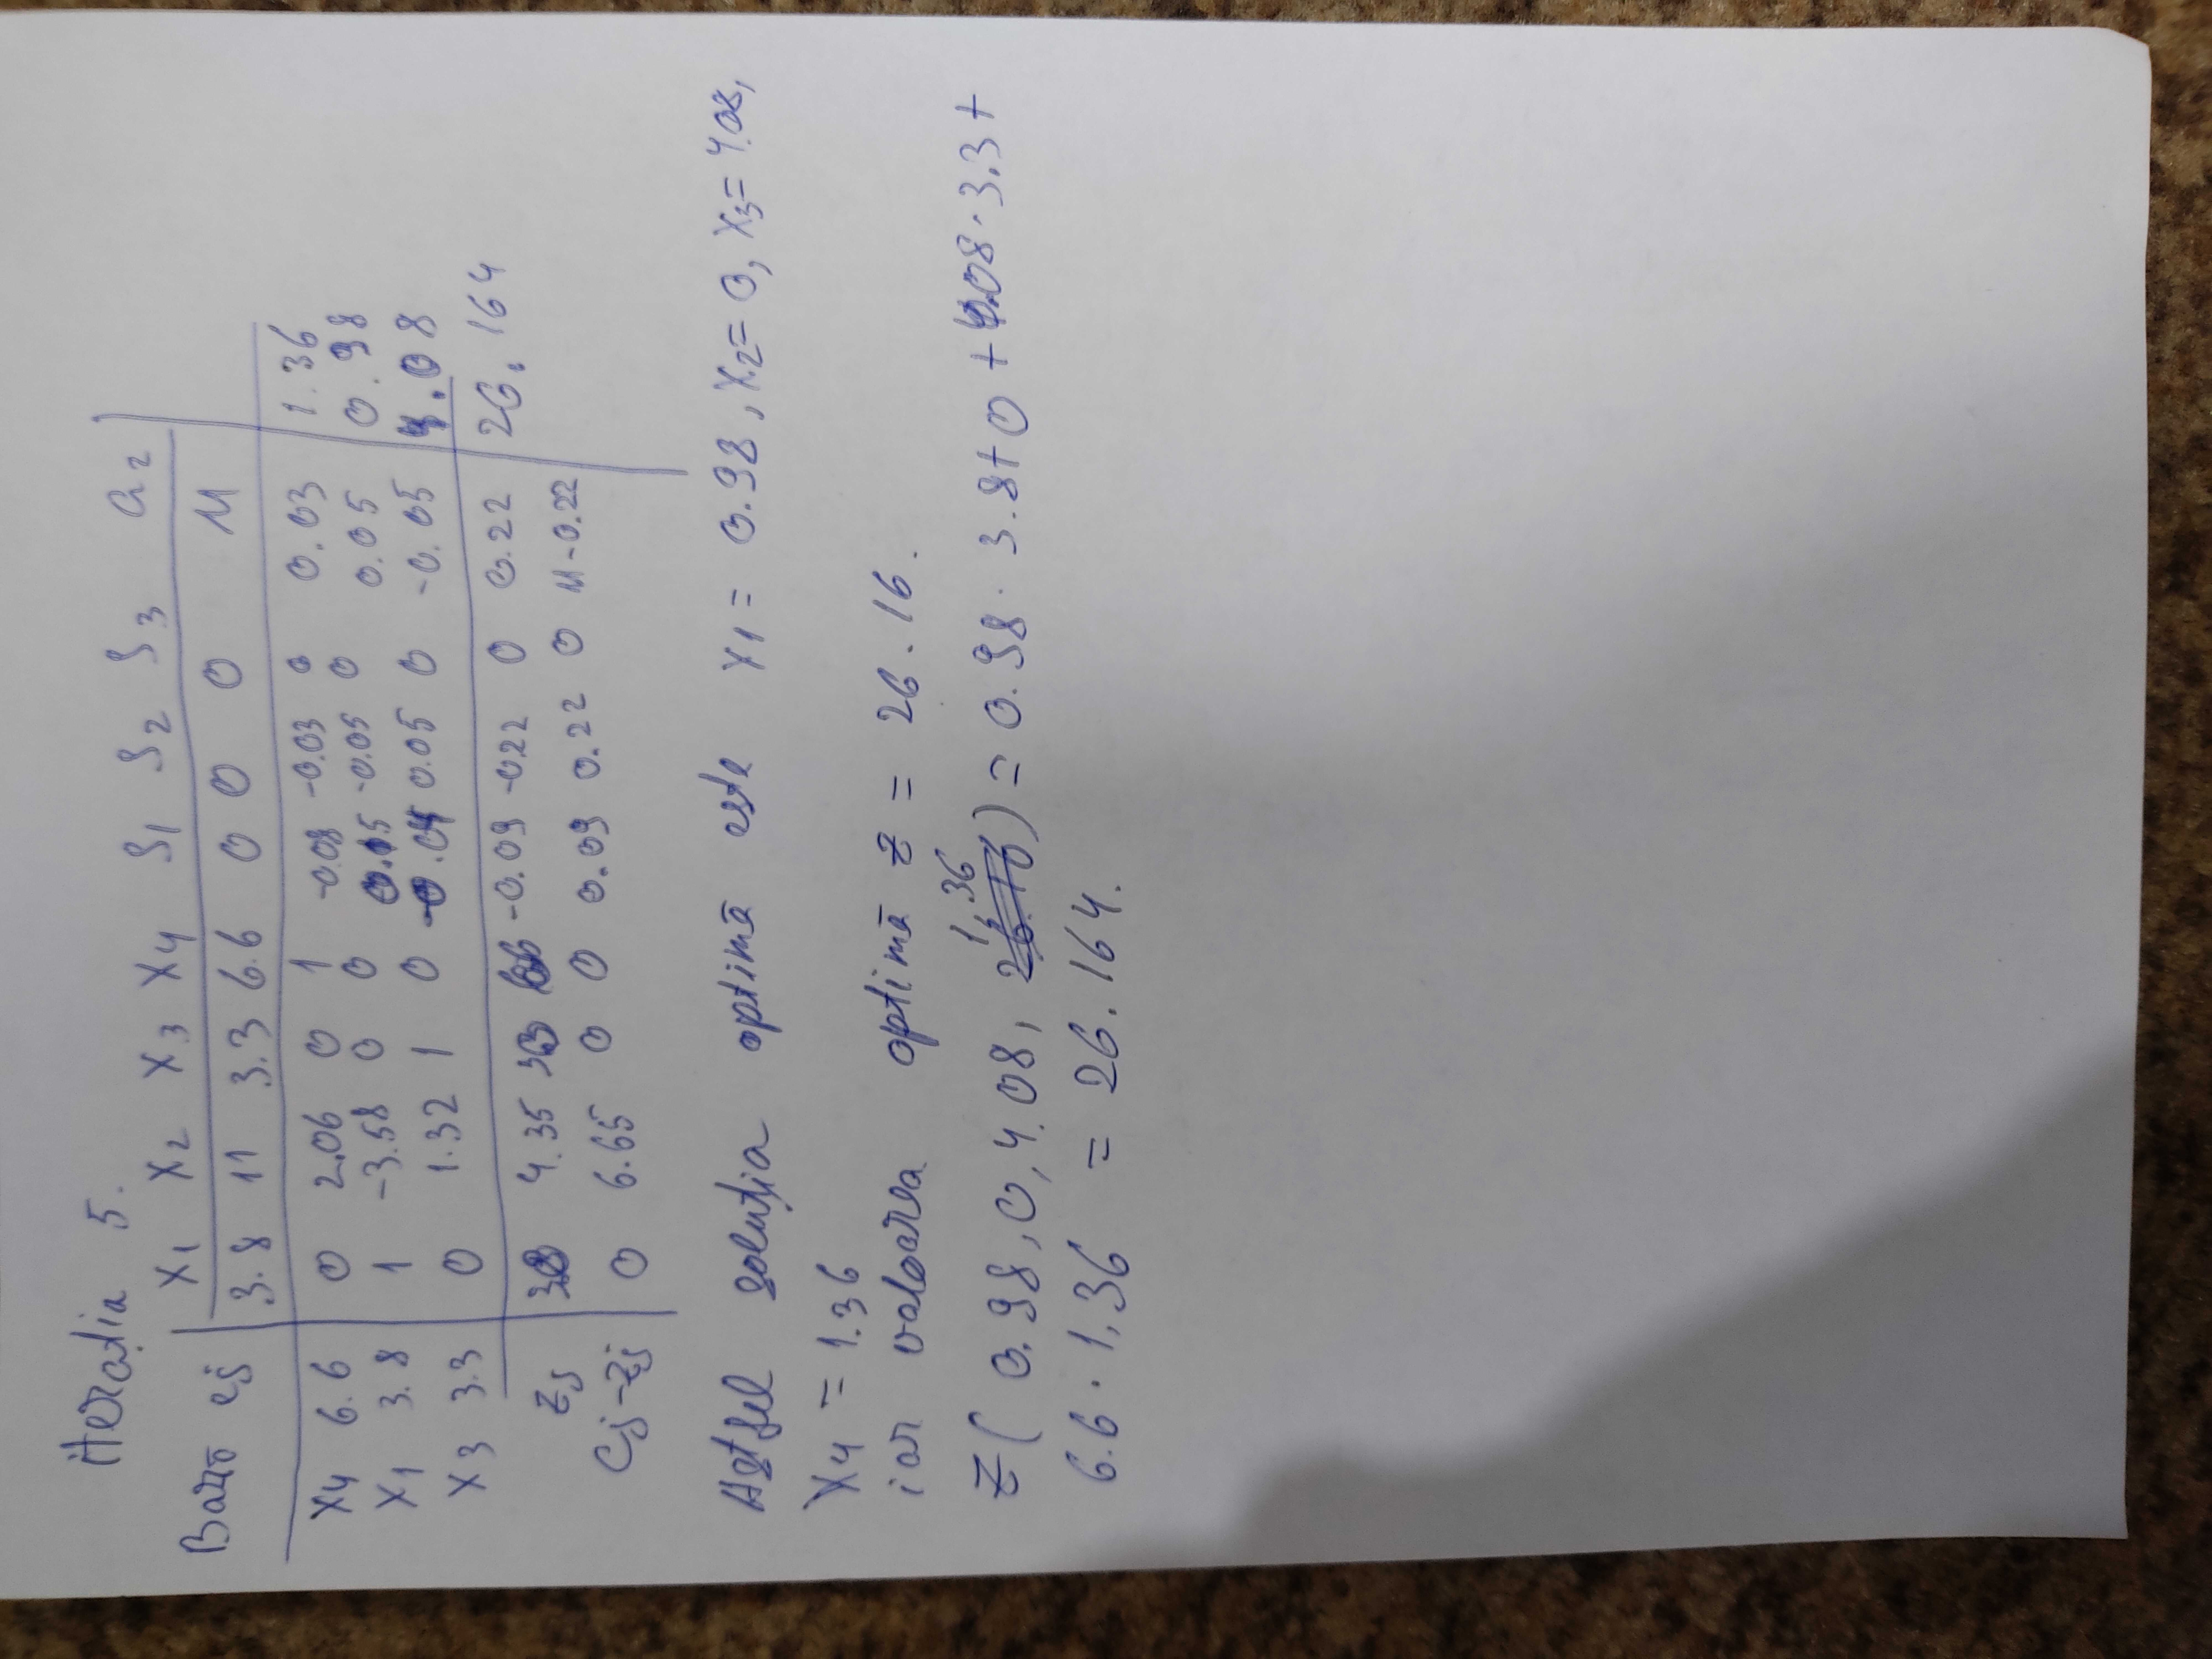
\includegraphics[width=22cm, angle =-90]{5}
\caption{Metoda simplex} 
\label{fig:5}
\end{center}
\end{figure}



\clearpage
\subsection*{PPL de maximizare – producție}
\paragraph{}
Compania \textbf{Chevrolet} dorește să obțină un venit maxim în urma producției de mașini. Modelele pe care aceasta companie le produce sunt Aveo, Colorado, Camaro, Suburban. Resursa limitată pentru producția acestor mașini este timpul pentru fiecare proces, este nevoie de 4 procese pentru a face o mașină. Datele problemei sunt date în tabelul de mai jos.

\paragraph{}
\begin{figure}[h]
\begin{center}
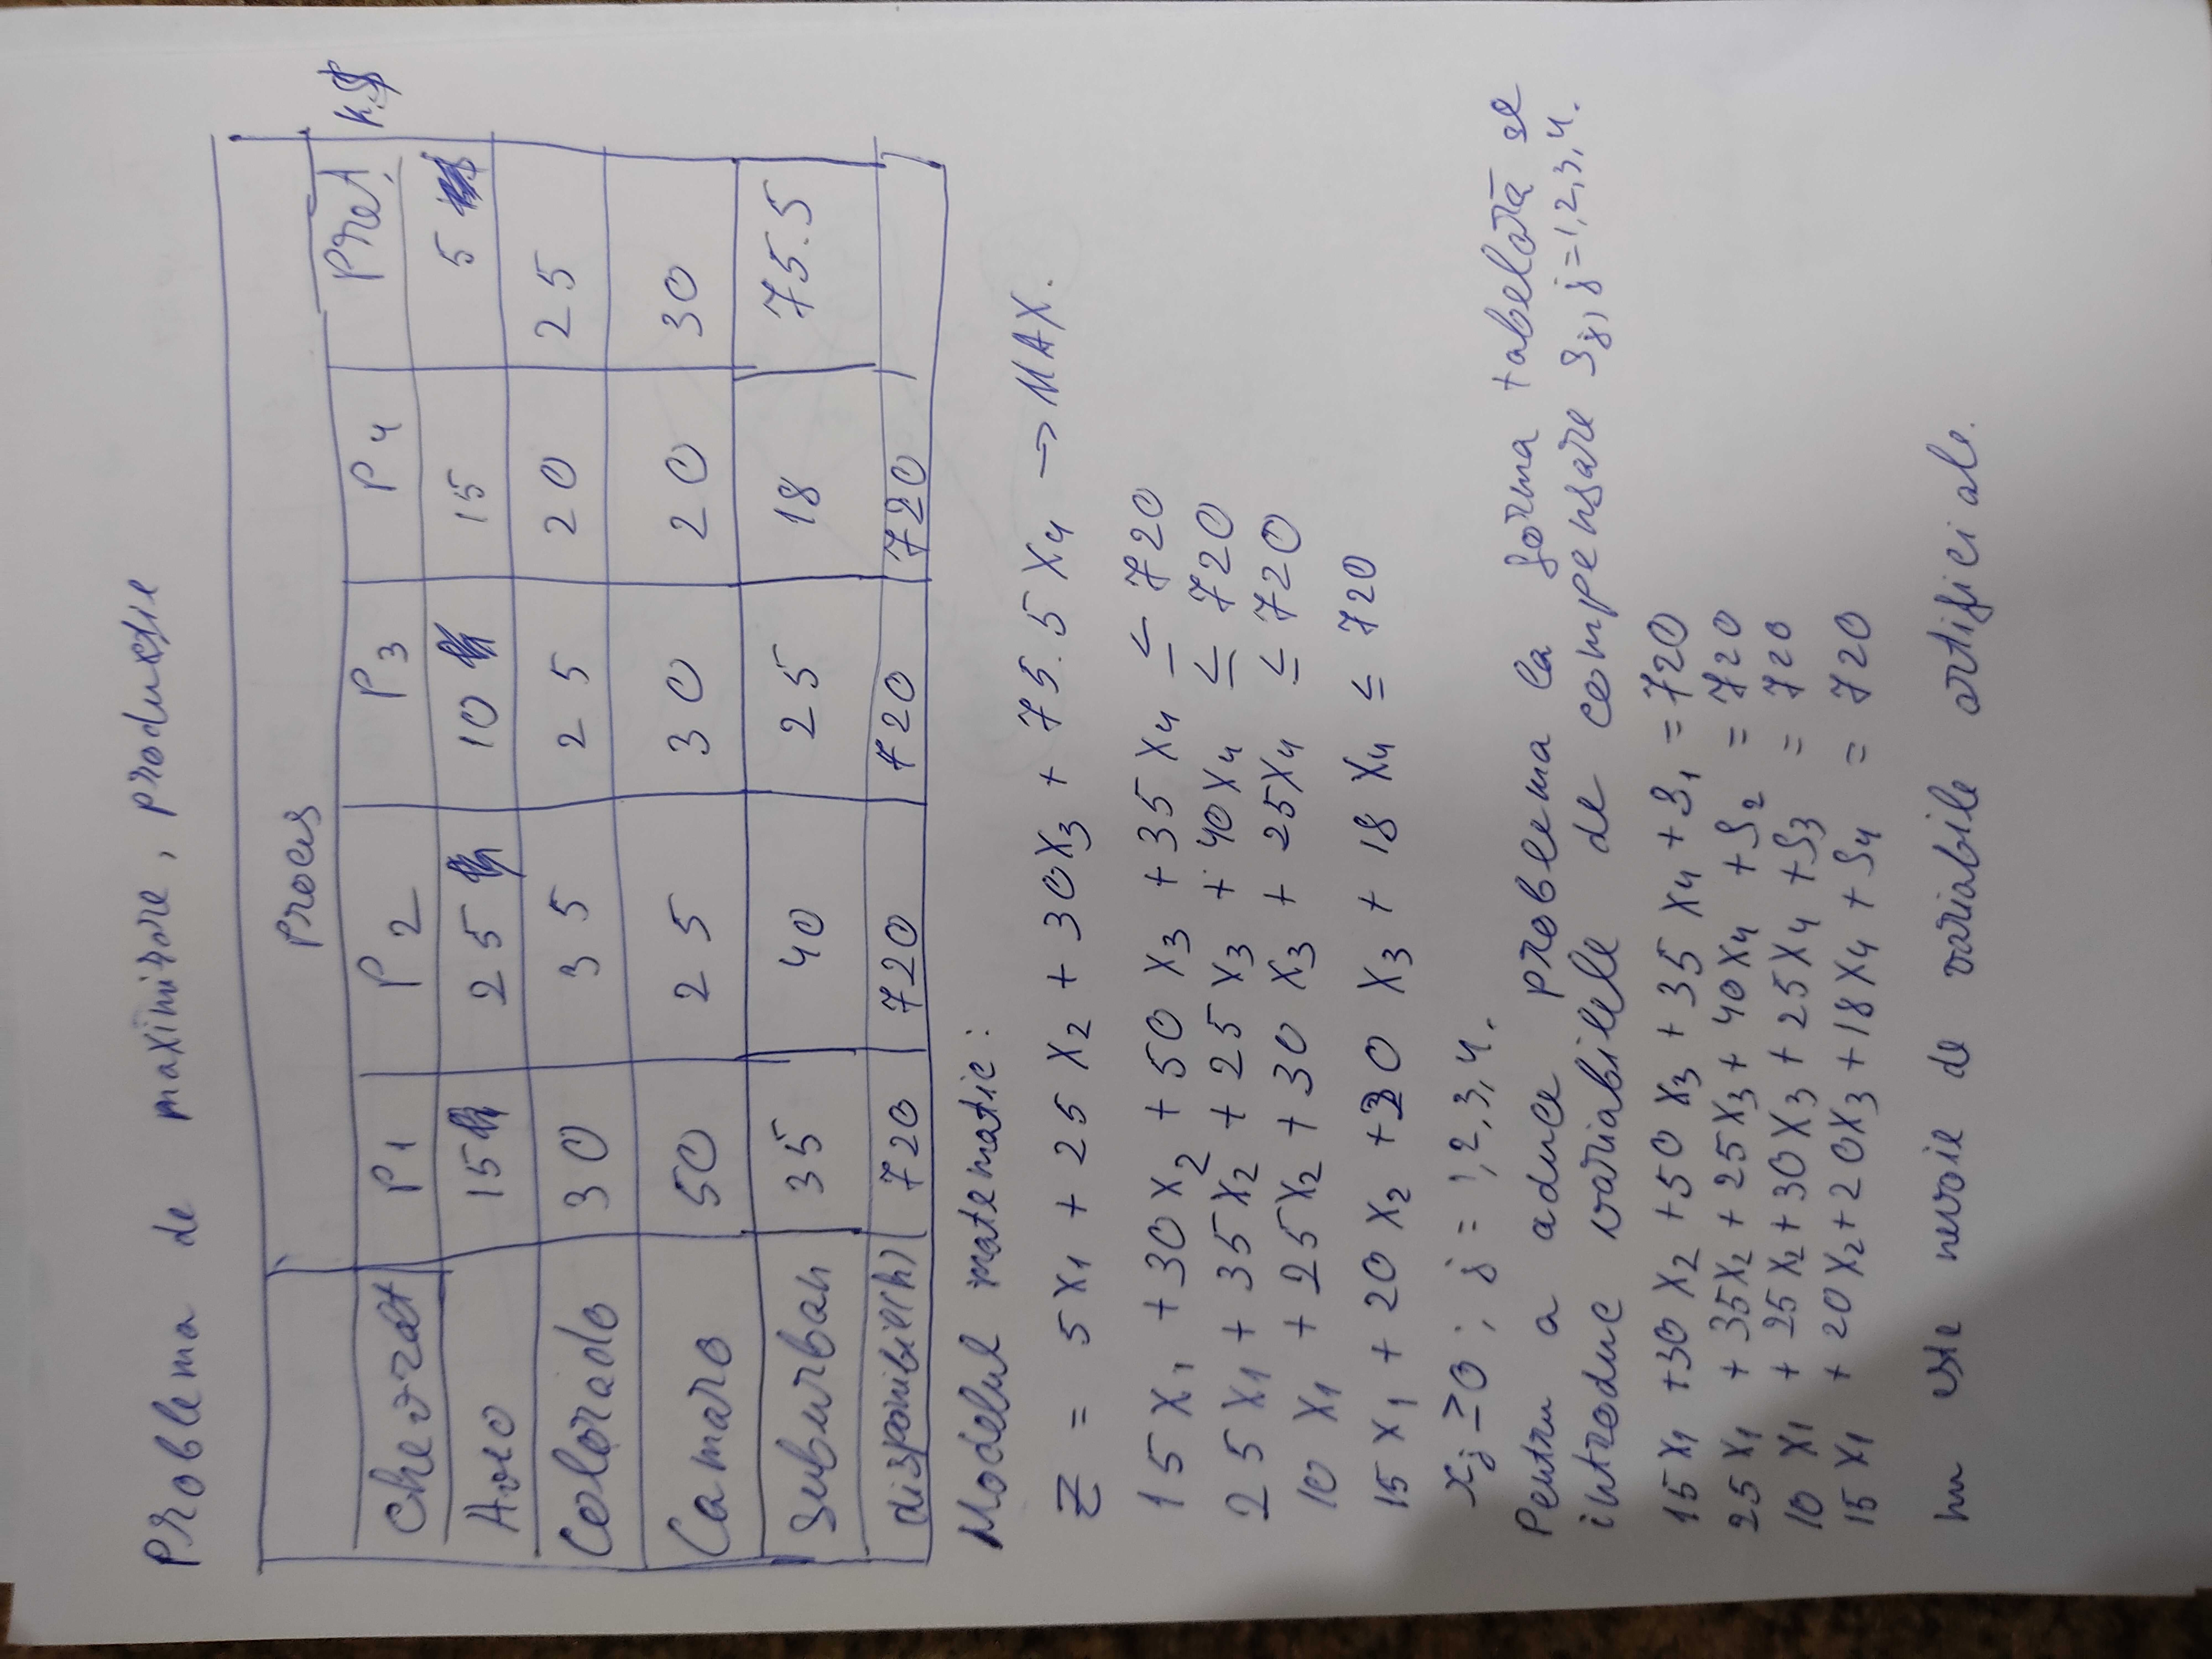
\includegraphics[width=22cm, angle =-90]{1}
\caption{Datele problemei și modelul matematic} 
\label{fig:1}
\end{center}
\end{figure}

\paragraph{}
\begin{figure}[h]
\begin{center}
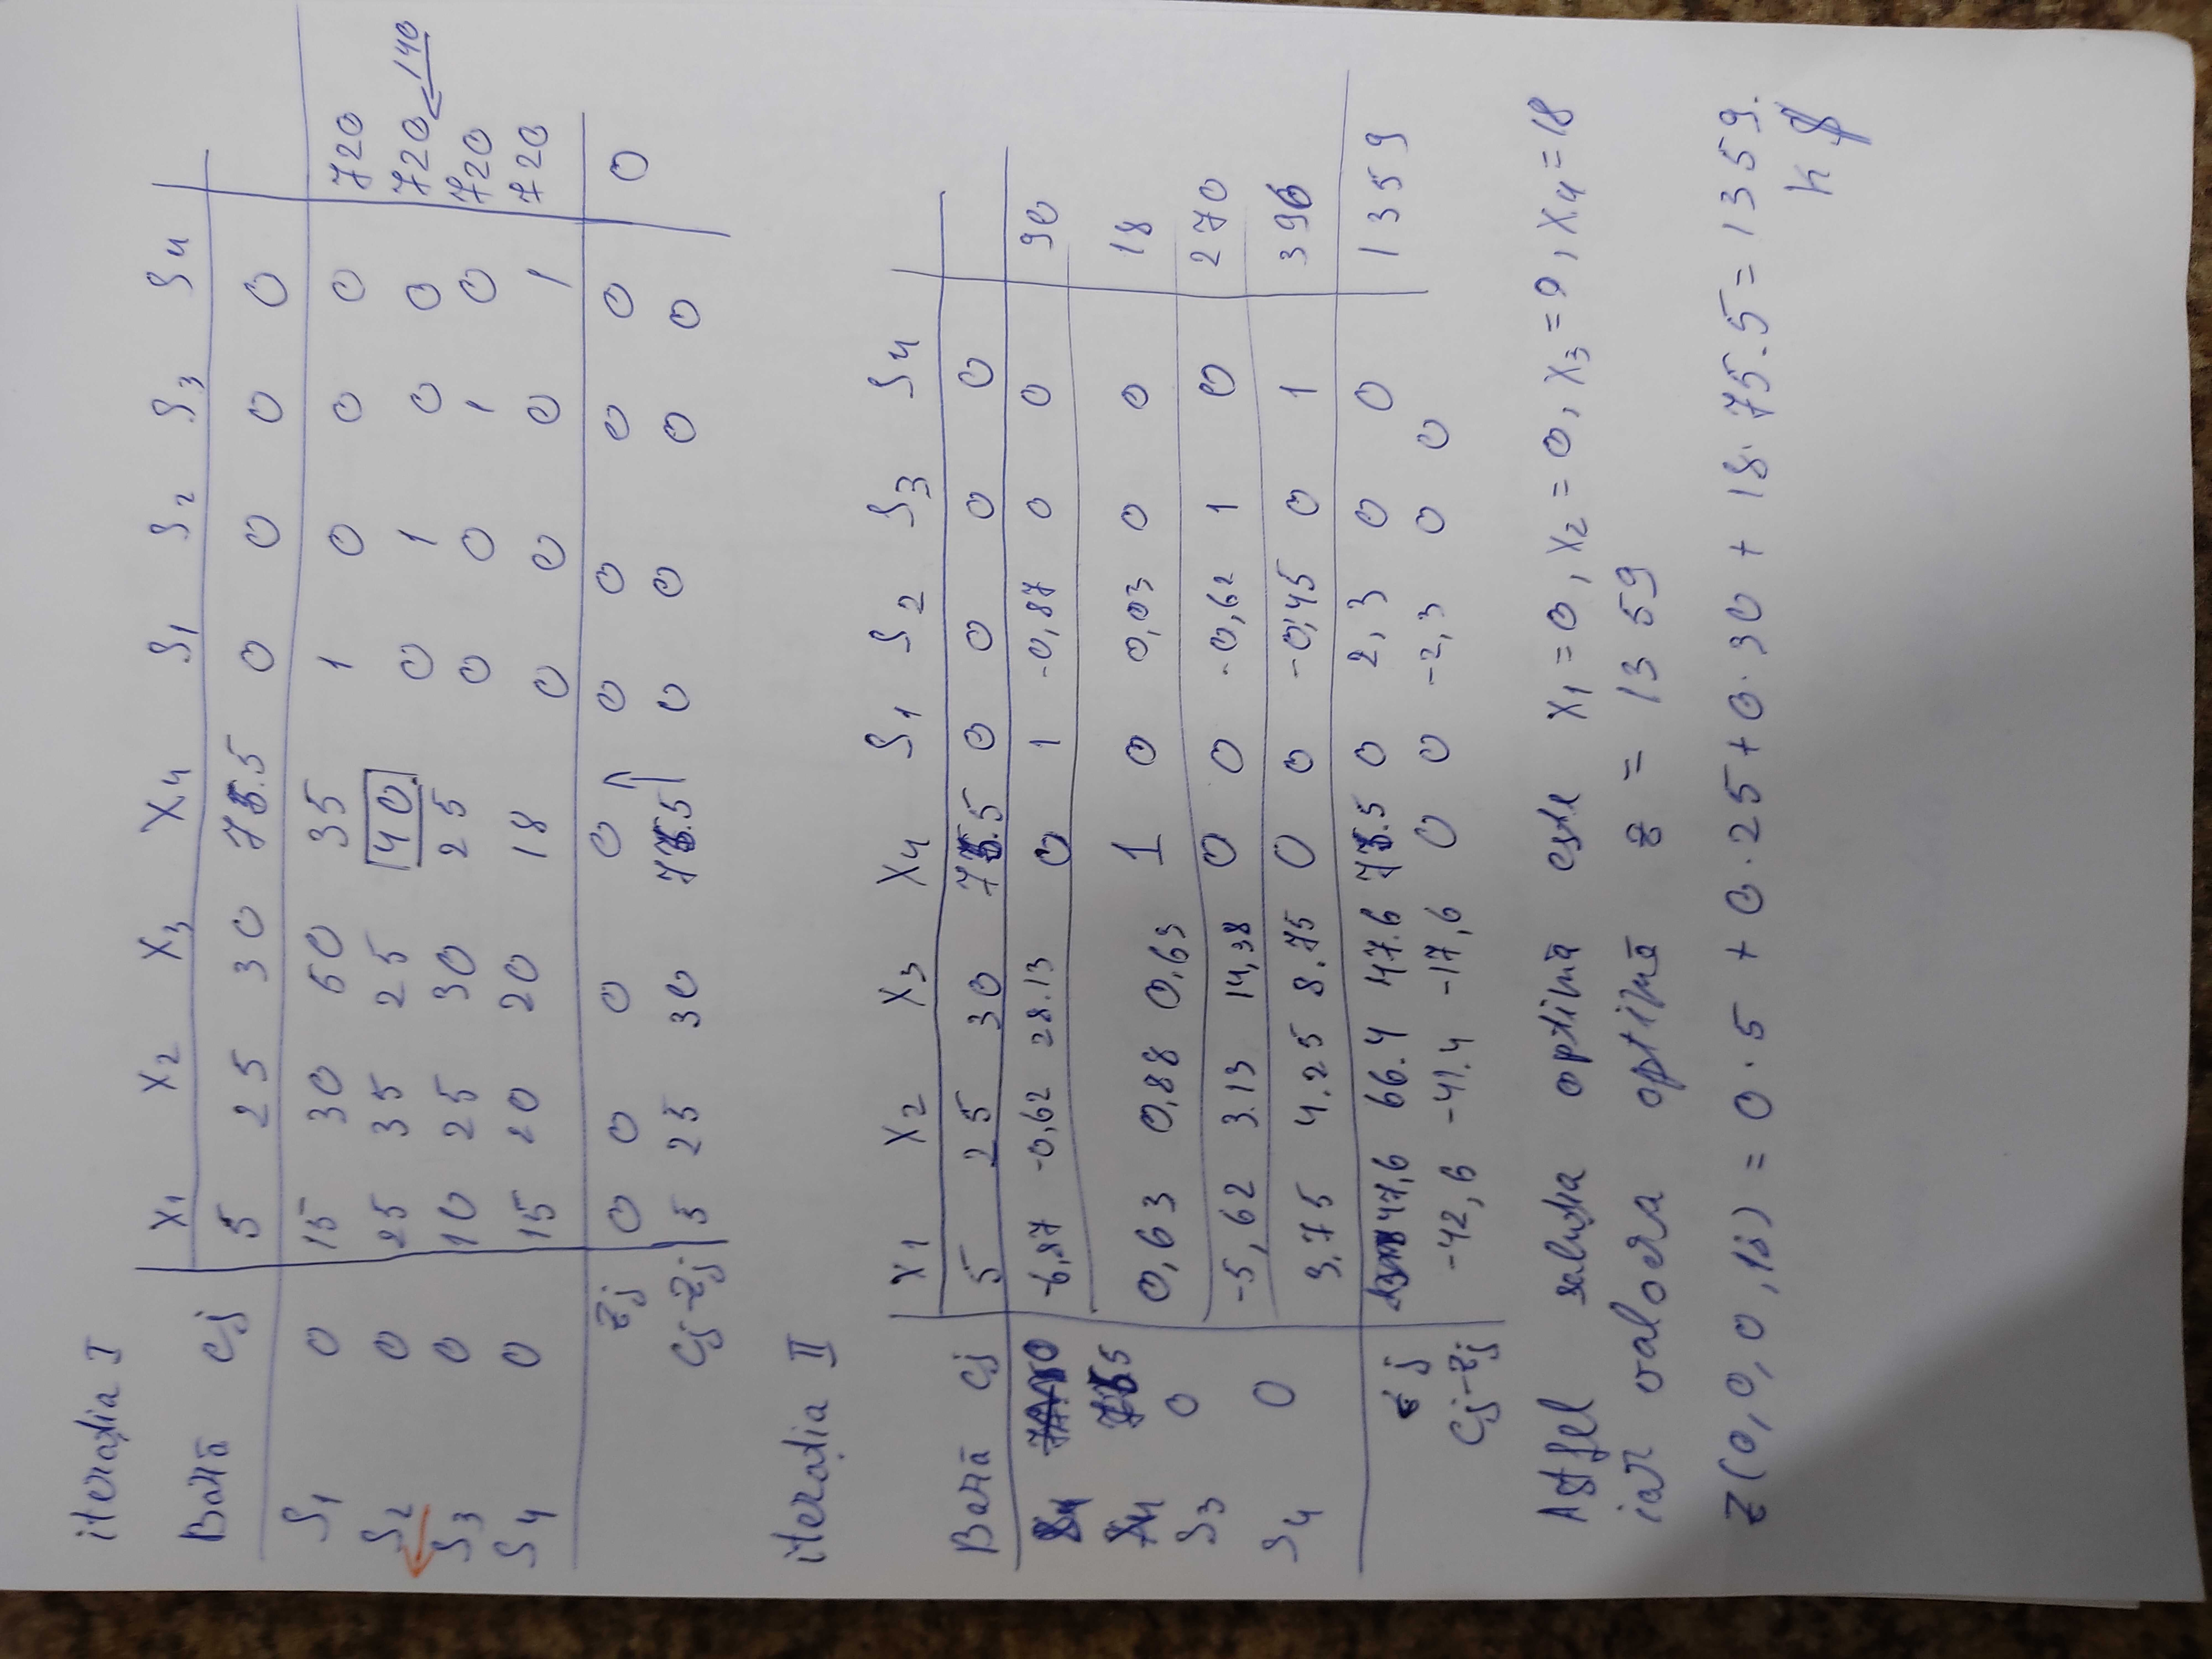
\includegraphics[width=22cm, angle =-90]{2}
\caption{Metoda simplex} 
\label{fig:2}
\end{center}
\end{figure}



\clearpage
\subsection*{Rezolvarea la nivel de cod}
\paragraph{}

\paragraph{}
\begin{figure}[h]
\begin{center}
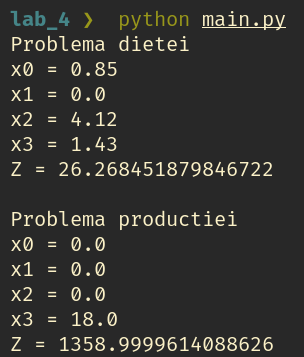
\includegraphics[width=12cm]{run}
\caption{Executarea codului care rezolva problema} 
\label{fig:1}
\end{center}
\end{figure}

\paragraph{Observații :}
În urma rezolvării problemei dietei pe foaie am obținut:
x\textsubscript{0} = 0.98, 
x\textsubscript{1} = 0, 
x\textsubscript{2} = 4.08,
x\textsubscript{2} = 1.36. 
Iar în urma rezolvarii la nivel de cod am obținut:
x\textsubscript{0} = 0.85,
x\textsubscript{1} = 0,
x\textsubscript{2} = 4.12,
x\textsubscript{2} = 1.43,
Rezultatul în urma minimizării pe foaie pare mai optim (26.164)
decât rezultatul aflat de calculator (26.268), însă acest lucru este
destul de imposibil de aceia voi considera că rezultatul aflat de calculator
a fost aflat într-un mod mai exact.
\\
\[ \Delta x_0 = 0.98 - 0.85 = 0.13 \]
\[ \Delta x_1 = 0    - 0    = 0 \]
\[ \Delta x_2 = 4.08 - 4.12 = 0.04 \]
\[ \Delta x_3 = 1.36 - 1.43 = 0.07 \]
\\
În urma rezolvării problemei de producție pe foaie și la nivel de cod am 
obținut aceleași rezultate:
x\textsubscript{0} = 0, 
x\textsubscript{1} = 0,
x\textsubscript{2} = 0,
x\textsubscript{2} = 18.

\clearpage
\paragraph{\large Concluzii:}\mbox{}\\

\subparagraph{}{
Am formulat două probleme de programare liniară una de amestec și una de producție.
Pentru problema de producție am încercat să aleg niște date cât mai realiste. Iar pentru problema dietei m-am informat despre valoarea nutritivă a diferitor alimente și prețul acestora.
}

\subparagraph{}{
Am utilizat mteoda tabelelor simplex pentru a rezolva aceste probleme. 
Pentru problema de producție rezolvarea a fost mai ușoară deoarece am avut doar două iterații. Pentru a rezolva această problemă a fost nevoie să utilizez doar variabile de compensare.
Problema dietei a fost ceva mai dificilă de oarece inițial plănuiam să utilizez mai multe variabile și constrângeri însă mărimea tabelului simplex ar fi fost prea mare și ar fi durat prea mult rezolvarea de mână, totuși această problemă s-a rezolvat prin 5 iterații. Pentru a rezolva această problemă a fost nevoie să utilizez și variabilele artificiale.
}


\subparagraph{}{
Pentru acest laborator am instalat si utilizat librăria \textbf{scipy} și anume funcția \textbf{linprog} care are ca argumente modelul matematic al problemei.
În urma consultării documentației acestei librării am descoperit ca funcția respectiva poate doar minimiza iar restricțiile pot fi doar '<=' și se explică cum putem transforma probleme cu date diferite în această formă.
Rezolvarea la nivel de cod nu a prezentat probleme și a fost de câteva ori mai rapidă decât metoda analitică pe foaie (anume scrisul codului).
}

\subparagraph{}{
Spre deosebire de metoda grafică, metoda tabelelor simplex permite optimizarea problemelor de programare liniară cu un număr mai mare de variabile, așa cum majoritatea problemelor din viața reală necesită mai mult de două variabile, (o dietă din 2 alimente ar if cam tristă) metoda de optimizare prin tabelele simplex este util de cunoscut.
}

\vfill
\subparagraph{}{
	\LaTeX
}


\begin{thebibliography}{9}
\bibitem{nutrition} http://www.foodnutritiontable.com/nutritions/
\bibitem{health} https://www.eatforhealth.gov.au/
\bibitem{linella} https://linella.md/ro

\appendix
\clearpage
\section*{Anexa main.py}
\lstinputlisting[language=python, frame=none]{../main.py}

\end{document}
